\chapter{Extension of the Rule-Based Lloyd Algorithm to 3D\label{chap:rbl}}
\section{Introduction}
    TODO
    \subsection{Motivation}
        Motivation in using RBL algo instead of some other algorithm
    \subsection{Problem Statement}
        Problems in the transition from 2d to 3d - algo needs to be fast 
    \subsection{Objectives}
        Extend the algorithm to 3D, do some experiments that are succesfull - show that algo works also for 3d taks
    \subsection{Chapter Overview}
        Summary of what this chapter covers

\section{Overview of RBL - TODO rename}

    \subsection{Overview}        
        The algorithm is a communication-less approach designed to navigate agents from point A to point B. 
        It relies on global positioning data, such as GPS or alternative methods for obtaining global coordinates, combined with sensor inputs that provide information about the agent's environment. 
        These sensors can include LiDAR, depth cameras, or standard cameras with estimation techniques, allowing the agent to detect and avoid obstacles or other agents. 
        The algorithm enables autonomous navigation without requiring direct communication between agents, making it suitable for scalable and decentralized applications.

    \subsection{Applications and Limitations in 2D}
        Modern robotics relies on the capability to navigate from point A to point B.
        Navigation plays a crucial role in various robotic applications, such as \ac{UGV}s, which are commonly used in manufacturing and logistics. 
        \ac{UGV}s typically follow predefined 2D trajectories guided by visual \cite{vision_navigation}, magnetic \cite{magnetic_navigation}, or LiDAR-based navigation \cite{lidar_navigation}. 
        Additionally, 2D navigation is widely employed in robotic vacuum cleaners, enabling them to systematically cover an area while avoiding obstacles.

        An obvious limitation for algorithms in 2D is scalability. 
        As the number of agents in a system increases, the complexity of managing their movements and coordination also grows significantly.
        Obstacle avoidance in 2D can also be less efficient compared to 3D environments, as agents have fewer options for evading obstacles. 
        In 3D, agents can change their altitude in addition to their horizontal trajectory, giving them more freedom to maneuver around obstacles.

    \subsection{Key principles}
        RBL, as presented in the original paper \cite{rbl_paper}, ensures convergence to the goal and provides sufficient conditions for achieving it. 
        The problem involves individual control of $N$ agents from their initial position $\mathbf{p}_i(0)$ toward a goal region, represented as circle.
        This goal region is denoted as $G(\mathbf{g}_i, r_g)$, where $\mathbf{g}_i$ is center and $r_g$ is radius of goal region. 
        The agent is progressing towards its designated destination, $\mathbf{d}_i$.
        Each agent is knows of its current position $\mathbf{p}_i$, encumbrance $\delta_i$, which determines safe space around agent.
        Additionally, each agent also knows the positions and encumbrances of its neighboring agents $\mathbf{\mathcal{N}_i}$, agent $j \in \mathbf{\mathcal{N}_i}$ if $||\mathbf{p}_i - \mathbf{p}_j|| \leq 2r_{s,i}$, where $r_{s,i}$ is denoted as half of the sensing radius of the i-th agent.
        For simplicity $r_{s,i}$ is considered to be same for all agents, therefore $r_{s,i} = r_s$. 

        The core objective of the algorithm is to minimize the coverage cost function, which accounts for the distribution of agents and obstacles over the environment. 
        This function is expressed as:
        \begin{equation}
            J_{cov}(\mathbf{p}) = \sum_{i=1}^{N} \int_{\mathcal{V}_i} \lVert\mathbf{q}-\mathbf{p}_i\rVert^2 \varphi_i (\mathbf{q})d\mathbf{q},
            \label{coverage_cost_function}
        \end{equation}
        where $\mathbf{p}_i$ is the position of agent $i$, $\mathcal{V}_i$ is the Voronoi cell of the i-th robot, $\lVert\mathbf{q}-\mathbf{p_i}\rVert^2$ is squared Euclidian distance between point in the mission space $\mathbf{q} \in \mathcal{Q}$ and agent's position $p_i$, 
        and $\varphi_i (\mathbf{q})$ is the weighting function.

        Voronoi cell is defined as: 
        \begin{equation}
            \mathcal{V}_i = \{q \in \mathcal{Q} \lvert \lVert \mathbf{q} - \mathbf{p}_i \rVert \leq \lVert q - \mathbf{p}_j \rVert, \forall j \neq i\}
        \end{equation}
        For visual representation see \reffig{fig:voronoi_2d}. 
        However, this standard definition of Voronoi cells does not take into account the physical space occupied by the agents, or their encumbrances. 
        To address this, a Modified Voronoi cell is introduced, which takes into account the encumbrances of agents.
        This modified version adjusts the boundaries of each Voronoi cell to account for the encumbrances of neighboring agents.
        The modified Voronoi cell definition is as follows:
        \begin{equation}
            \tilde{V}_i = 
            \begin{cases}
            \{ \mathbf{q} \in Q \mid \| \mathbf{q} - \mathbf{p}_i \| \leq \| \mathbf{q} - \mathbf{p}_j \| \}, & \text{if } \Delta_{ij} \leq \frac{\| \mathbf{p}_i - \mathbf{p}_j \|}{2} \\
            \{ \mathbf{q} \in Q \mid \| \mathbf{q} - \mathbf{p}_i \| \leq \| \mathbf{q} - \tilde{\mathbf{p}}_j \| \}, & \text{otherwise},
            \end{cases}
        \end{equation}
        $\forall j \in \mathcal{N}_i$, where $\Delta_{ij} = \delta_i + \delta_j$ and $\tilde{\mathbf{p}}_j = \mathbf{p}_j + 2(\Delta_{ij} - \frac{\| \mathbf{p}_i - \mathbf{p}_j \|}{2})\frac{ \mathbf{p}_i - \mathbf{p}_j }{\| \mathbf{p}_i - \mathbf{p}_j \|}$.
        Together with cell $\mathcal{S}_i$ defined as: 
        \begin{equation}
            \mathcal{S}_i = \{\mathbf{q} \in \mathcal{Q} | \| \mathbf{q} - \mathbf{p}_i \| \leq r_{s,i}\}
        \end{equation}
        the cell $\mathcal{A}_i$ is obtained as $\mathcal{A}_i = \tilde{V}_i \cap \mathcal{S}_i$.

        Convergence to goal region $G(\mathbf{g}_i, r_g )$ depends on the choice of weighting function that assigns weights to points $\mathbf{q}$ in the mission space $\mathcal{Q}$.
        The weighting function $\varphi_i(\mathbf{q})$ is defined as follows: 
        \begin{equation}
            \varphi_i(\mathbf{q}) = \exp\left(-\frac{\|\mathbf{q} - \mathbf{d}_i\|}{\beta_i}\right),
        \end{equation}
        where $\beta_i$ is the weighting factor for points $\mathbf{q}$, and $\mathbf{d}_i$ represents the current destination of the agent. 
        The destination is computed as follows:
        \begin{equation}
            \mathbf{d}_i = \mathbf{p}_i + R(\theta)(\mathbf{g}_i - \mathbf{p}_i)
        \end{equation}
        where $R$ is the azimuthal rotation.
        Rules: 
        \begin{itemize}
            \item \textbf{Weighting rule}
                \begin{equation}
                    \dot{\beta}_i(A_i) = 
                    \begin{cases}
                        -k & \text{if } \beta_i > \beta_{min} \land \|\mathbf{c}_{A_i} - \mathbf{p}_i\| < d_1 \land \|\mathbf{c}_{A_i} - \mathbf{c}_{\mathcal{S}_i}\| > d_2  \\
                        0  & \text{if } \beta_i > \beta_{min} \land \|\mathbf{c}_{A_i} - \mathbf{p}_i\| < d_1 \land \|\mathbf{c}_{A_i} - \mathbf{c}_{\mathcal{S}_i}\| > d_2  \\
                        -(\beta_i - \beta_i^D) & \text{otherwise}
                    \end{cases}
                \end{equation}
                where the first case decreases $\beta_i$ over time, the second case ensures that $\beta_i$ does not decrease below its minimum threshold $\beta_{min}$ (saturation) and the third case provides a general update rule when the previous conditions are not met.
            \item \textbf{Azimuth rule}
                \begin{equation}
                    \dot{\theta}_i = 
                    \begin{cases}
                        k  & \text{if } \theta < \frac{\pi}{2} \land \|\mathbf{c}_{\mathcal{A}_i} - \mathbf{c}_{\mathcal{S}_i}\| > d_4 \land \|\mathbf{p}_i - \mathbf{c}_{\mathcal{A}_i}\| > d_3 \\
                        -k & \text{if } \theta > 0 \land \neg (\|\mathbf{c}_{\mathcal{A}_i} - \mathbf{c}_{\mathcal{S}_i}\| > d_4 \land \|\mathbf{p}_i - \mathbf{c}_{\mathcal{A}_i}\| > d_3) \\
                        0  & \text{otherwise}
                    \end{cases}
                \end{equation}
                where the first case increases $\theta_i$ over time, the second case ensures that $\theta_i$ converges back when the distance constraints are not satisfied, and the third case keeps $\theta_i$ unchanged.
            \item \textbf{Azimuth reset rule}
                \begin{equation}
                    \theta = 0 \text{if } \theta = \frac{\pi}{2} \land \| \mathbf{p}_i - \mathbf{\overline{c}}_{\mathcal{A}_i} \|    
                \end{equation}
                where $\mathbf{\overline{c}}_{\mathcal{A}_i}$ represents the centroid computed from the cell $\mathcal{A}_i$, which is weighted using the unrotated destination, meaning $\mathbf{d}_i = \mathbf{g}_i$.
        \end{itemize}
        Weighted centroid is computed as follows:        
        \begin{equation}
            \mathbf{c}_{\mathcal{A}_i} = \frac{\int_{\mathcal{A}_i} \mathbf{q} \varphi_i(\mathbf{q}) \, d\mathbf{q}}{\int_{\mathcal{A}_i} \varphi_i(\mathbf{q}) \, d\mathbf{q}},
        \end{equation}
        where \( \mathbf{q} \) represents the point in mission space, and \( \varphi_i(\mathbf{q}) \) is a weighting function. 

        By applying the previously defined rules and computations, the RBL algorithm successfully guides agents movement toward the goal.
        However, these rules focus solely on rotating the centroid $\mathcal{A}_i$ in the azimuthal plane. 
        To enhance performance in a fully three-dimensional space, additional rules are required to account for elevation adjustments. 
    \subsection{Agressivity of RBL alog TODO rename}
        modification of cell A so it can move closer to objects - cwvd parameters

\section{Extension of the RBL algorithm to 3D}
    \subsection{Motivation for 3D Extension}
        In many practical applications, agents must operate in three-dimensional spaces, considering not only horizontal movement but also vertical positioning.
        A 3D extension is necessary to navigate complex environments that feature obstacles in all directions.
        In 2D, agents are restricted to a flat plane, which simplifies navigation but limits the ability to interact with objects and environments that exist in the third dimension.
        The ability to utilize vertical space can enhance energy efficiency, as agents can optimize their paths by ascending or descending to avoid obstacles or to find more favorable environmental conditions, such as discovering more open space.
        The transition from 2D to 3D also opens up possibilities for more advanced movement strategies, such as navigating through multi-level environments or optimizing trajectories by utilizing vertical space.  
        Moreover, the use of 3D models allows for more accurate representations of real-world scenarios, where elevation plays a crucial role in decision-making and task execution.


    \subsection{Differences between 2D and 3D}
        The primary distinction in the 3D extension is that each goal region is now represented as a sphere rather than a circle.  
        Similarly, the sensing cell $\mathcal{S}_i$ is also modeled as a sphere instead of a circle, allowing for a more accurate representation of the \ac{UAV}'s perception in three-dimensional space.  
        This change introduces a key modification when defining $\tilde{V}_i$: in the 2D case, a line was sufficient to slice the sensing region, whereas in 3D, a plane must be computed to properly segment the spherical sensing cell. 
        
        \begin{figure}[H]
            \centering
            \subfloat[Euclidean Voronoi Diagram in 2D] {
            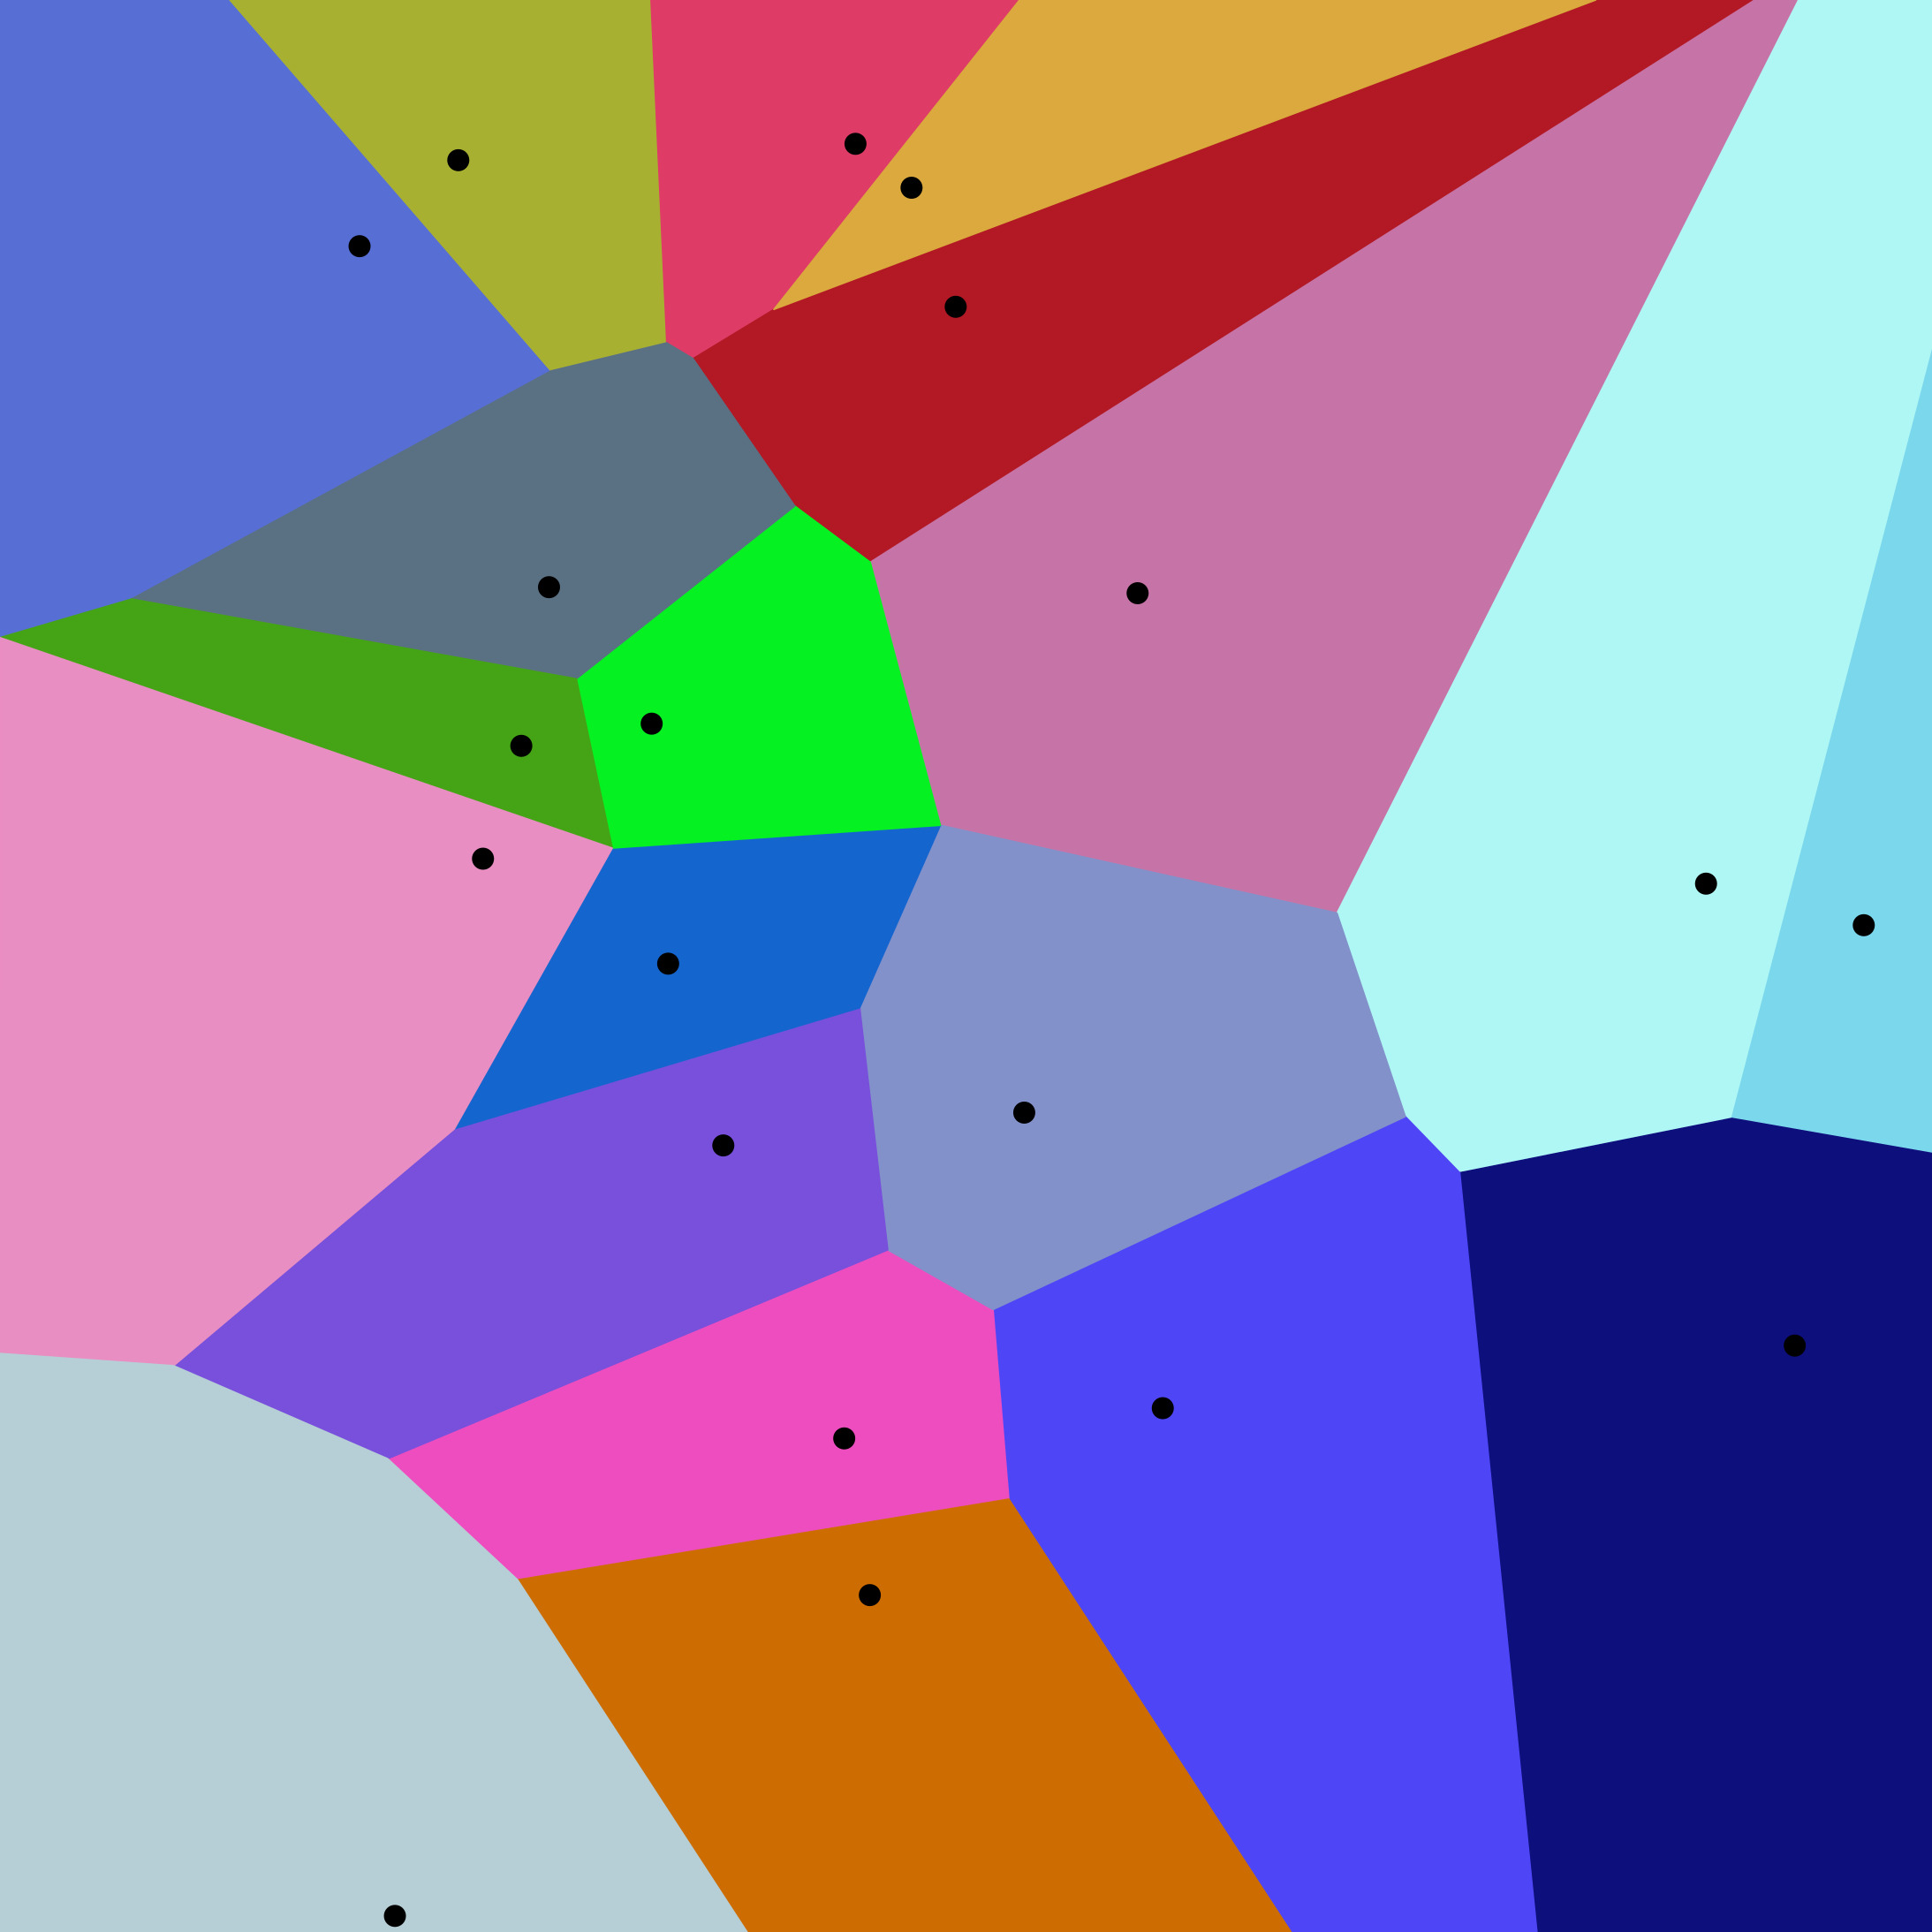
\includegraphics[width=0.48\textwidth, height=0.48\textwidth]{./fig/diagrams/Euclidean_Voronoi_diagram.jpg}
            \label{fig:voronoi_2d}
            }
            \subfloat[Euclidean Voronoi Diagram in 3D] {
            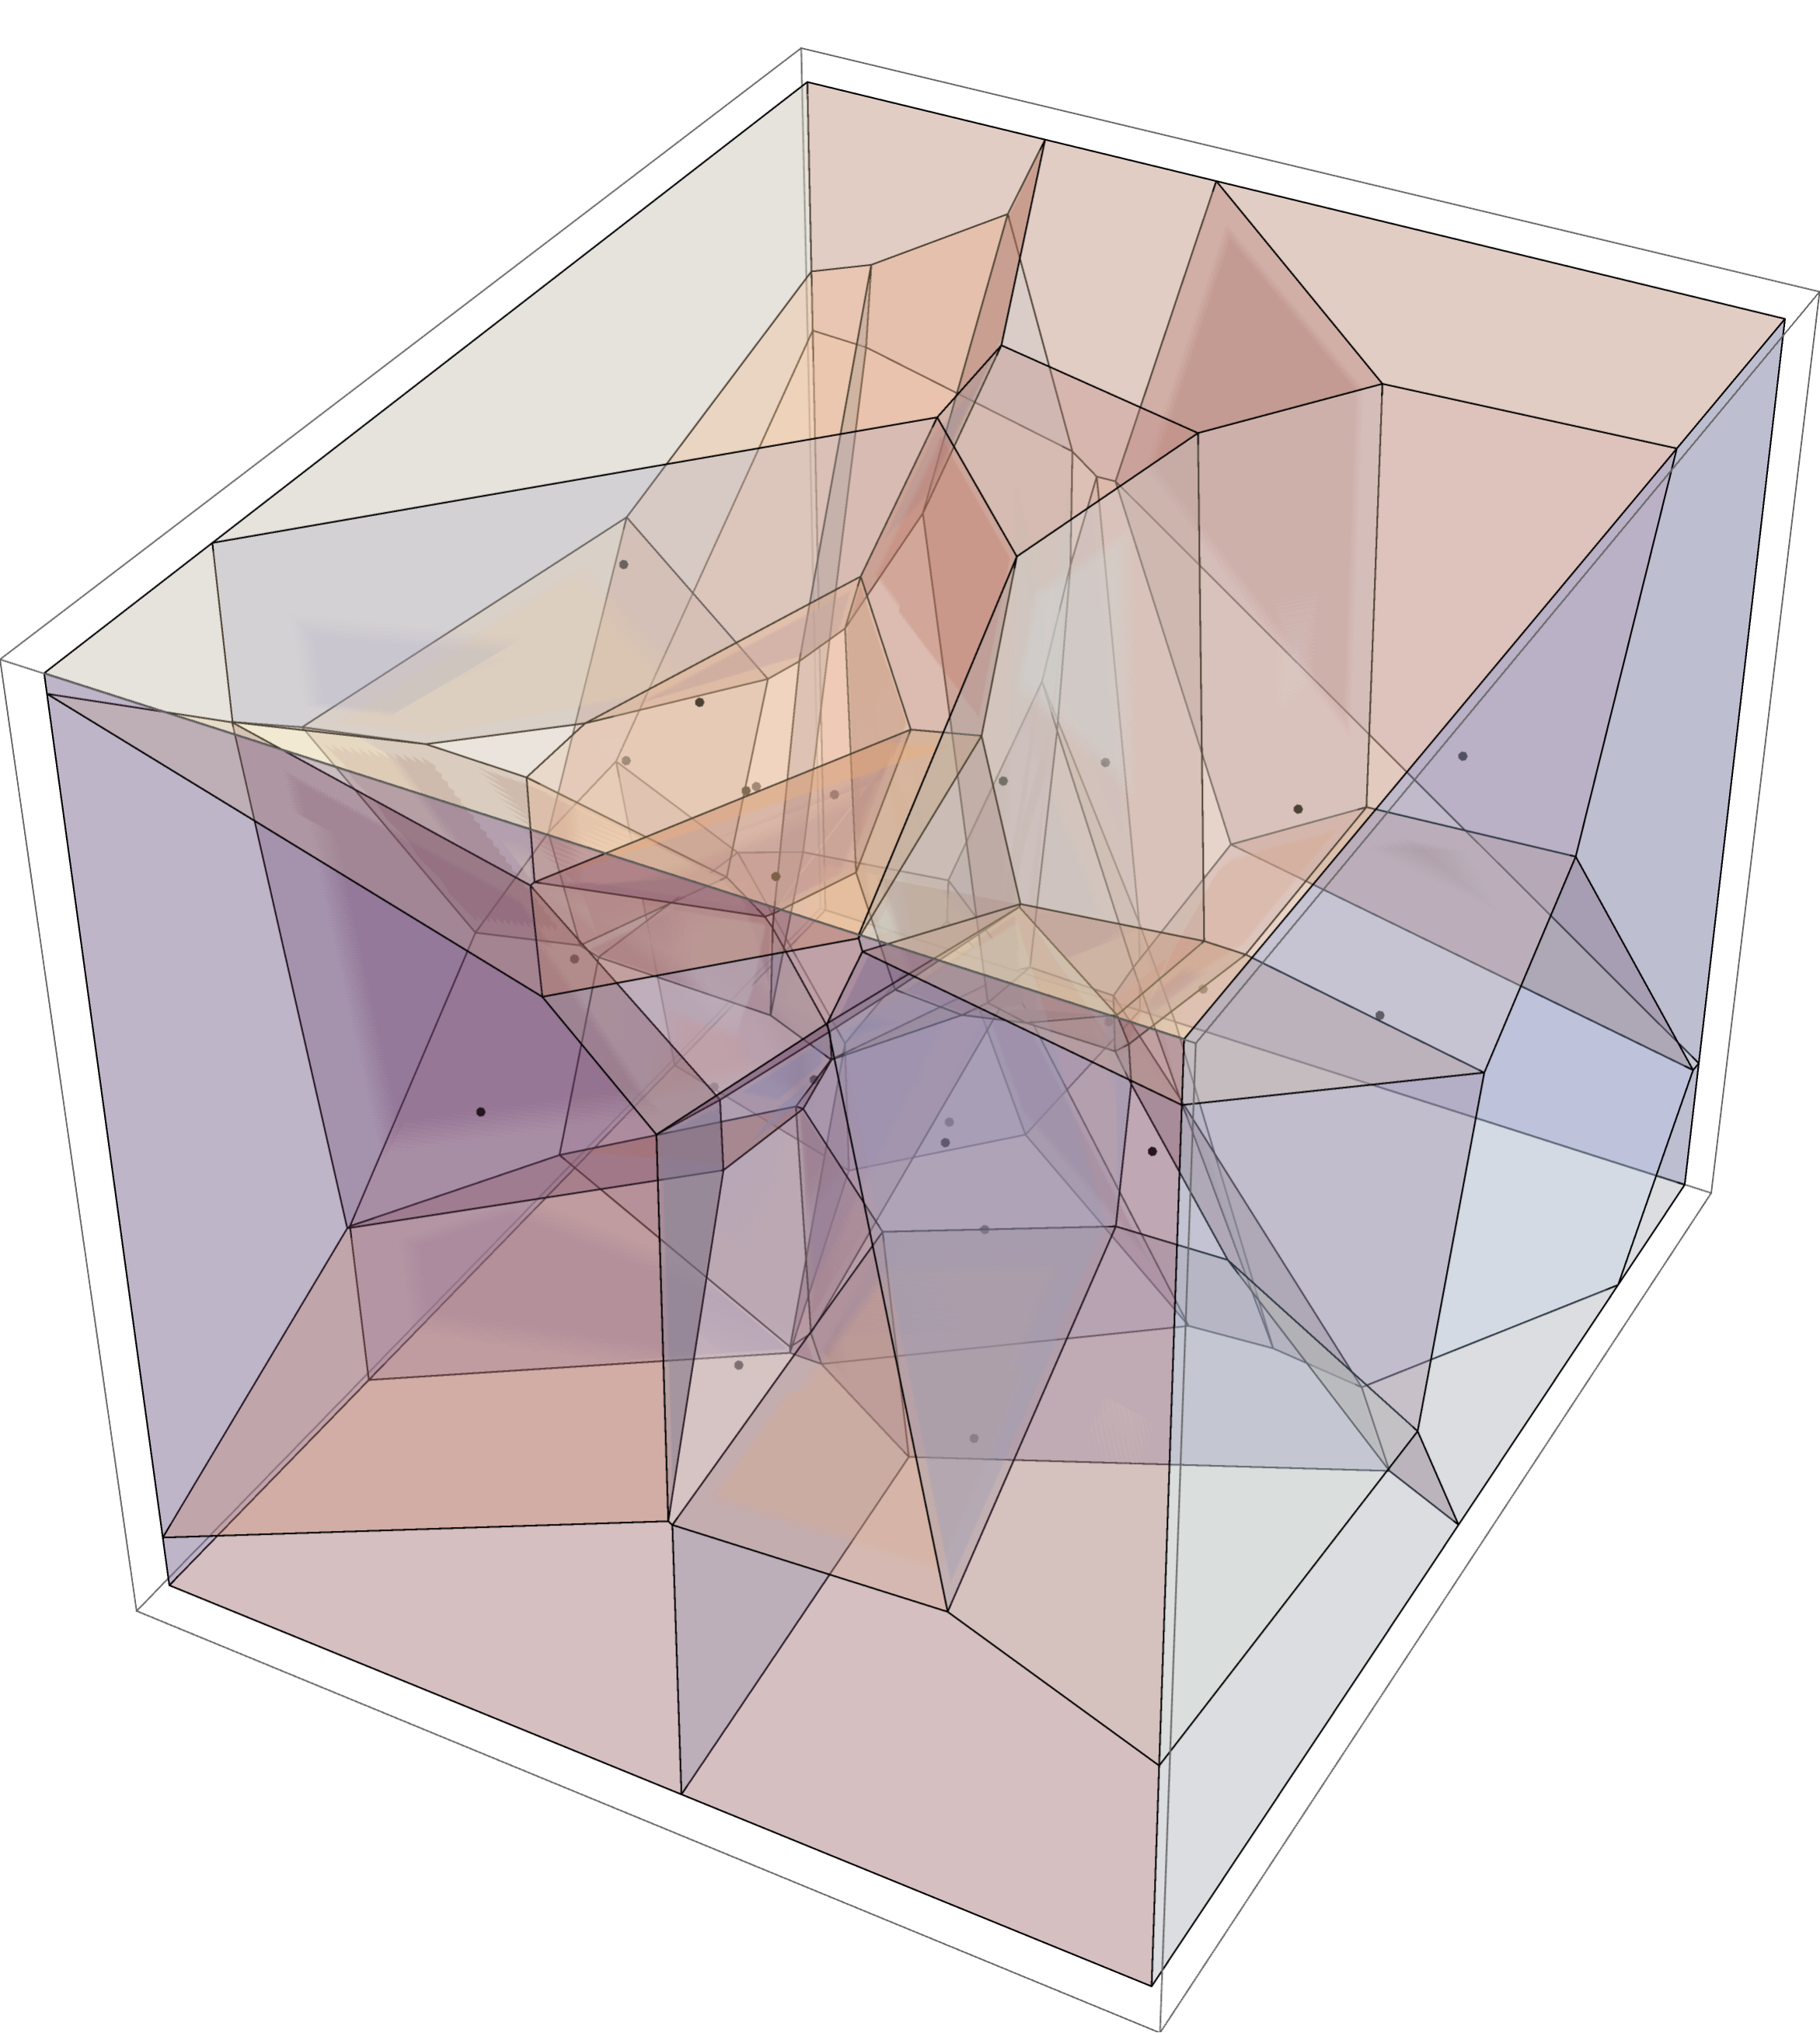
\includegraphics[width=0.48\textwidth, height=0.48\textwidth]{./fig/diagrams/Euclidian Voronoi diagram 3d.png}
            \label{fig:voronoi_3d}
            }
            \caption{
                (a) an example of 20 Voronoi cells in 2D \cite{Voronoi2d} (b) 25 Voronoi cells in 3D \cite{Voronoi3d}
            }
            \label{fig:voronoi_diagrams}
        \end{figure}
    
    \subsection{Additional Constraints and Modifications}
        For the 3D case, several modifications are introduced. 
        Firstly, $Z_{clipping}$ is applied to each sensing cell $\mathcal{S}_i$, constraining it within the vertical limits defined by $\text{min}_z$ and $\text{max}_z$:

        \begin{equation}
            \mathcal{S}_i = \left\{\mathbf{q} \in \mathcal{Q} \mid \|\mathbf{q} - \mathbf{p}_i\| \leq r_{s,i}, \quad \text{min}_z \leq q_z \leq \text{max}_z \right\}
        \end{equation}

        where $\text{min}_z$ and $\text{max}_z$ define the vertical bounds within which the sensing region $\mathcal{S}_i$ is restricted. 
        This ensures that the \ac{UAV} cannot exceed these limits, as it follows the computed centroid \( \mathbf{c}_{V_i} \). 
        By constraining the sensing radius, the \ac{UAV} remains confined within the specified region, preventing it from moving outside the vertical interval $\text{min}_z$ to $\text{max}_z$.

        Secondly, $Z_{rule}$ is intorduced to enhance \ac{UAV} avoidance. Rule rotates computed centroid by $\phi$

        \begin{equation}
            \dot{\phi}_i(A_i) =
            \begin{cases}
                \text{sgn}(\omega_i) \cdot dt, & \text{if } \|\mathbf{c}_{A_i} - \mathbf{p}_i\|_z < d_6 \land \|\mathbf{c}_{S_i} - \mathbf{c}_{A_i}\|_z > d_5 \\ 
                                               & \lor (\|\mathbf{p}_i - \mathbf{c}_{S_i}\|_{xy} - \|\mathbf{p}_i - \mathbf{c}_{A_i}\|_{xy}) > d_7, \\
                -\text{sgn}(\phi_i) \cdot dt,  & \text{otherwise.}
            \end{cases}
        \end{equation}
        
        where the directional influence \(\omega_i\) is given by a weighted combination:
        
        \begin{equation}
            \omega_i = \frac{w_1 \cdot \|\mathbf{c}_{S_i} - \mathbf{p}_i\|_z + w_2 \cdot \left(\frac{\theta_i}{\pi} - 1\right)}{w_1 + w_2},
        \end{equation}
        
        with 
        
        \begin{equation}
            \theta_i = \text{atan2}(g_x - p_{ix}, g_y - p_{iy}),
        \end{equation}
        
        ensuring it remains in \([0, 2\pi]\). The weights \(w_1\) and \(w_2\) balance the contribution of vertical distance and directional influence.
        
        \paragraph{Convergence Back to Zero}  
        If no condition for modification is met, \(\phi\) converges back to zero:
        
        \begin{equation}
            \dot{\phi}_i = 
            \begin{cases}
                -dt, & \phi_i > 0, \\
                dt, & \phi_i < 0, \\
                0, & \phi_i = 0.
            \end{cases}
        \end{equation}
        
        \paragraph{Constraint on \(\phi\)}  
        A constraint ensures that vertical avoidance does not increase separation:
        
        \begin{equation}
            \phi_i = 0, \quad \text{if } |\phi_i| = \frac{\pi}{4} \land \|\mathbf{p}_i - \mathbf{c}_{S_i}\|_z > \|\mathbf{p}_i - \mathbf{c}_{A_i}\|_z.
        \end{equation}
        
        This ensures that if vertical modification makes the drone farther from the reference, it is reset.

\section{Simulation and Results Analysis}

Describtion of simulation enviroment, used tools, Describtion of few simulation scenarios and result analysis.
    \subsection{Simulation Enviroment}
        The term 'agent' refers to the \ac{UAV}s used in the simulation.
        For this simulation, I relied on the framework provided by \cite{mrs_uav_system}
        Each \ac{UAV} obtains its global position from the ROS simulator, RViz.
        The positions of other \ac{UAV}s were estimated using blinking LEDs mounted on each \ac{UAV}, based on the method outlined in \cite{uvdd1}.
        Below, I list some relevant constraints for each \ac{UAV}:
        \begin{table}[h]
            \centering
            \renewcommand{\arraystretch}{1.1}
            \begin{tabular}{|l|c|}
                \hline
                \textbf{Parameter} & \textbf{Value} \\ \hline
                    Maximal horizontal velocity [\SI{}{\meter\per\second}] & 4.0 \\ \hline
                    Horizontal acceleration [\SI{}{\meter\per\second\squared}] & 2.0 \\ \hline
                    Maximal ascending velocity [\SI{}{\meter\per\second}] & 2.0 \\ \hline
                    Vertical ascending acceleration [\SI{}{\meter\per\second\squared}] & 1.0 \\ \hline
                    Maximal descending velocity [\SI{}{\meter\per\second}] & 2.0 \\ \hline
                    Vertical descending acceleration [\SI{}{\meter\per\second\squared}] & 1.0 \\ \hline
                \end{tabular}
                \caption{Motion constraints of the \ac{UAV}.}
            \label{tab:uav_constraints}
        \end{table}
    \subsection{Simulation Scenarios}
        Several experiments were conducted to evaluate and ensure the safe behavior of the \ac{UAV}s during interactions. 
        Different sets of \ac{UAV}s were used in these experiments, with N = 5, 10, and 15, and data was collected from them for analysis. 
        Each \ac{UAV} was first flown from ground to its initial position, and once all \ac{UAV}s were in their starting positions, the RBL algorithm was initiated.

        For most agent interactions, experiments were conducted in both circular and spherical formations, with the circular formation being initially conducted in \cite{rbl_paper}. 
        The circular formation was chosen as it promotes more predictable and consistent interactions between agents, as opposed to random initial positions and goal locations, which could lead to less structured or less frequent interactions. 
        Similarly, the spherical formation was introduced to extend the experiment into 3D, providing a more comprehensive test scenario. 
        Both structured formations help to better evaluate the performance of the RBL algorithm in environments where agents are more likely to encounter each other.
        The \ac{UAV}s were evenly distributed along the perimeter of the circle or the surface of the sphere. 
        The goal position was placed on the opposite side of the circle or sphere. 
        The radius of both the circle and the sphere was set to 5 meters.
        
        TODO table of parameters used for this experiment.
        Sensing radius $r_s$ = 4.5m, update rate 10 Hz, encumbrance 0.5 m, d1 = d3 = d5 = 0.5, d2 = d4 = d6 = 1.0.
        For $z_{clipping}$ - $min_z$ = 1.0 m, $max_z$ = 10.0


        In the next tables 
        
        \subsection{N = 5 circular}
            \begin{table}[H]
                \centering
                \renewcommand{\arraystretch}{1.2}
                \begin{tabular}{|l|c|c|c|c|c|}
                \hline
                                            & \( SR \ [\%] \) & \( \overline{L} \ [\mathrm{m}] \) & \( \overline{t} \ [\mathrm{s}] \) & \( \overline{t}_{\text{max}} \ [\mathrm{s}] \) & \( \overline{v} \ [\mathrm{m/s}] \)     \\ \hline
                RBL 2D                      & 100.00          & 21.06 $\pm$ 0.10                  & 25.15 $\pm$ 0.21                  & 25.15 $\pm$ 0.19                               & 0.83 $\pm$ 0.01                         \\ \hline
                RBL 3D                      & 100.00          & 20.77 $\pm$ 0.29                  & 26.04 $\pm$ 0.51                  & 26.79 $\pm$ 0.27                               & 0.79 $\pm$ 0.02                         \\ \hline
                RBL 3D\(_{\text{clipped}}\) & 100.00          & 20.60 $\pm$ 0.24                  & 26.73 $\pm$ 0.47                  & 27.39 $\pm$ 0.28                               & 0.77 $\pm$ 0.02                         \\ \hline
                RBL 3D\(_z\)                & 100.00          & 20.97 $\pm$ 0.52                  & 25.54 $\pm$ 0.97                  & 26.72 $\pm$ 0.60                               & 0.81 $\pm$ 0.03                         \\ \hline
                \end{tabular}
            \end{table}

        \subsection{N = 10 circular}
            \begin{table}[H]
                \centering
                \renewcommand{\arraystretch}{1.2}
                \begin{tabular}{|l|c|c|c|c|c|}
                \hline
                                            & \( SR \ [\%] \) & \( \overline{L} \ [\mathrm{m}] \) & \( \overline{t} \ [\mathrm{s}] \) & \( \overline{t}_{\text{max}} \ [\mathrm{s}] \) & \( \overline{v} \ [\mathrm{m/s}] \)     \\ \hline
                RBL 2D                      & 100.00          & 22.95 $\pm$ 1.64                  & 30.79 $\pm$ 2.28                  & 34.73 $\pm$ 0.77                               & 0.74 $\pm$ 0.07                         \\ \hline
                RBL 3D                      & 100.00          & 22.22 $\pm$ 0.89                  & 30.05 $\pm$ 2.61                  & 34.39 $\pm$ 4.19                               & 0.73 $\pm$ 0.05                         \\ \hline
                RBL 3D\(_{\text{clipped}}\) & 100.00          & 22.31 $\pm$ 0.69                  & 30.22 $\pm$ 1.83                  & 33.22 $\pm$ 0.93                               & 0.73 $\pm$ 0.04                         \\ \hline
                RBL 3D\(_z\)                & 100.00          & 22.38 $\pm$ 0.88                  & 28.80 $\pm$ 2.30                  & 32.35 $\pm$ 1.25                               & 0.77 $\pm$ 0.05                         \\ \hline
                \end{tabular}
            \end{table}
        
        \subsection{N = 15 circular}
        \begin{table}[H]
            \centering
            \renewcommand{\arraystretch}{1.2}
            \begin{tabular}{|l|c|c|c|c|c|}
            \hline
                                        & \( SR \ [\%] \) & \( \overline{L} \ [\mathrm{m}] \) & \( \overline{t} \ [\mathrm{s}] \) & \( \overline{t}_{\text{max}} \ [\mathrm{s}] \) & \( \overline{v} \ [\mathrm{m/s}] \)     \\ \hline
            RBL 2D                      & 100.00          & 23.56 $\pm$ 1.75                  & 33.89 $\pm$ 2.48                  & 38.75 $\pm$ 1.45                               & 0.69 $\pm$ 0.06                         \\ \hline
            RBL 3D                      & 100.00          & 22.36 $\pm$ 0.97                  & 30.65 $\pm$ 3.07                  & 35.77 $\pm$ 3.72                               & 0.72 $\pm$ 0.07                         \\ \hline
            RBL 3D\(_{\text{clipped}}\) & 100.00          & 22.32 $\pm$ 0.81                  & 30.69 $\pm$ 2.61                  & 34.50 $\pm$ 0.47                               & 0.72 $\pm$ 0.06                         \\ \hline
            RBL 3D\(_z\)                & 100.00          & 22.64 $\pm$ 0.95                  & 29.67 $\pm$ 2.54                  & 34.27 $\pm$ 0.88                               & 0.76 $\pm$ 0.06                         \\ \hline
            \end{tabular}
        \end{table}
    
        \subsection{N = 10 sphere}
            \begin{table}[H]
                \centering
                \renewcommand{\arraystretch}{1.2}
                \begin{tabular}{|l|c|c|c|c|c|}
                \hline
                                            & \( SR \ [\%] \) & \( \overline{L} \ [\mathrm{m}] \) & \( \overline{t} \ [\mathrm{s}] \) & \( \overline{t}_{\text{max}} \ [\mathrm{s}] \) & \( \overline{v} \ [\mathrm{m/s}] \)     \\ \hline
                RBL 2D                      & 100.00          & 00.00 $\pm$ 0.00                  & 00.00 $\pm$ 0.00                  & 00.00 $\pm$ 0.00                               & 0.00 $\pm$ 0.00                         \\ \hline
                RBL 3D                      & 100.00          & 00.00 $\pm$ 0.00                  & 00.00 $\pm$ 0.00                  & 00.00 $\pm$ 0.00                               & 0.00 $\pm$ 0.00                         \\ \hline
                RBL 3D\(_{\text{clipped}}\) & 100.00          & 00.00 $\pm$ 0.00                  & 00.00 $\pm$ 0.00                  & 00.00 $\pm$ 0.00                               & 0.00 $\pm$ 0.00                         \\ \hline
                RBL 3D\(_z\)                & 100.00          & 00.00 $\pm$ 0.00                  & 00.00 $\pm$ 0.00                  & 00.00 $\pm$ 0.00                               & 0.00 $\pm$ 0.00                         \\ \hline
                \end{tabular}
            \end{table}


    \subsection{Practical Experiment Setup}
            
    \subsection{Comparisons}

\section{Summary and Key Insights}

    Recap of modifications. Faced challenges and solutions applied
